\documentclass[conference]{IEEEtran}
\IEEEoverridecommandlockouts
% The preceding line is only needed to identify funding in the first footnote. If that is unneeded, please comment it out.
\usepackage{cite}
\usepackage{amsmath,amssymb,amsfonts}
\usepackage{algorithmic}
\usepackage{graphicx}
\usepackage{textcomp}
\usepackage{xcolor}
\usepackage{hyperref}
\usepackage{tcolorbox}
\tcbuselibrary{skins}

% Define styles for user and assistant boxes
\newtcolorbox{userbox}{colback=blue!5,colframe=blue!40!black,title=User}
\newtcolorbox{assistantbox}{colback=gray!10,colframe=black,title=Assistant}

\def\BibTeX{{\rm B\kern-.05em{\sc i\kern-.025em b}\kern-.08em
    T\kern-.1667em\lower.7ex\hbox{E}\kern-.125emX}}
\begin{document}

\title{HASHIRU: Hierarchical Agent System for Hybrid Intelligent Resource Utilization}

\author{\IEEEauthorblockN{Kunal Pai}
\IEEEauthorblockA{\textit{UC Davis} \\
kunpai@ucdavis.edu}
\and
\IEEEauthorblockN{Parth Shah}
\IEEEauthorblockA{\textit{Independent Researcher} \\
helloparthshah@gmail.com}
\and
\IEEEauthorblockN{Harshil Patel}
\IEEEauthorblockA{\textit{UC Davis} \\
hpppatel@ucdavis.edu}
\and
\IEEEauthorblockN{Saisha Shetty}
\IEEEauthorblockA{\textit{UC Davis} \\
spshetty@ucdavis.edu}
}

\maketitle

\section{Introduction}\label{sec:introduction}

Rapid advancements in Large Language Models (LLMs) are reshaping Artificial Intelligence (AI) with profound capabilities in language understanding, generation, reasoning, and planning \cite{brown2020language, devlin2019bert, raffel2020exploring}. This progress drives the development of autonomous AI agents, shifting focus from single to Multi-Agent Systems (MAS) where collaborative teams tackle complex problems beyond individual scope \cite{dorri2018multi, wooldridge2009introduction}. Collaborative MAS show significant potential in diverse domains like scientific discovery \cite{boiko2023emergent}, software engineering \cite{qian2023communicative}, data analysis, and strategic decision-making \cite{wang2023decision}. The increasing complexity of tasks, demonstrated by benchmarks requiring advanced mathematical reasoning (e.g., GSM8K \cite{cobbe2021gsm8k}, SVAMP \cite{patel2021svamp}), coding (e.g., HumanEval \cite{chen2021codex}, CoDocBench \cite{pai2024codocbench}), and graduate-level technical knowledge \cite{phan2025humanitysexam}, highlights the need for agentic systems to effectively coordinate diverse cognitive resources \cite{wen2024benchmarkingcomplexinstructionfollowingmultiple}.

Despite this potential, contemporary agentic frameworks face significant limitations. Many are \textbf{rigid}, relying on predefined roles and static structures hindering adaptation to dynamic tasks \cite{zhang2023building}. \textbf{Resource obliviousness} is common; systems often lack mechanisms to monitor and optimize computational resources like API costs, memory, and CPU load, leading to inefficiency, especially when scaling or deploying in resource-constrained environments \cite{park2023generative}. This is often worsened by reliance on powerful, costly proprietary cloud LLMs. \textbf{Model homogeneity}, defaulting to a single powerful LLM for all sub-tasks, misses efficiency gains from a diverse ecosystem including smaller, specialized, or local models \cite{zhou2023agents}. While \textbf{tool use} is fundamental \cite{yao2022react, parisi2022talm}, agents' ability to autonomously \textbf{create and integrate new tools} remains limited, restricting dynamic extension and self-improvement without human intervention \cite{wang2023voyager}.

To address these challenges, we introduce \textbf{HASHIRU (Hierarchical Agent System for Hybrid Intelligent Resource Utilization)}, a novel MAS framework enhancing flexibility, resource efficiency, and adaptability. HASHIRU employs a hierarchical structure led by a central ``CEO'' agent dynamically managing specialized ``employee'' agents instantiated on demand. A core tenet is its \textbf{hybrid intelligence} approach, strategically prioritizing smaller (e.g., 3B--7B), locally-run LLMs (often via Ollama \cite{ollama}) for cost-effectiveness and efficiency. While prioritizing local resources, the system flexibly integrates external APIs and potentially more powerful models when justified by task complexity and resource availability, under the CEO's management.

The primary contributions are:
\begin{enumerate}
    \item A novel MAS architecture combining \textbf{hierarchical control} with \textbf{dynamic, resource-aware agent lifecycle management} (hiring/firing). This management is governed by computational budget constraints (cost, memory, concurrency) and includes an economic model with hiring/firing costs to discourage excessive churn.
    \item A \textbf{hybrid intelligence model} prioritizing cost-effective, local LLMs while adaptively incorporating external APIs and larger models, optimizing the efficiency-capability trade-off.
    \item An integrated mechanism for \textbf{autonomous API tool creation}, allowing dynamic functional repertoire extension.
    \item An \textbf{economic model} (hiring/firing fees) for agent management, promoting efficient resource allocation and team stability.
\end{enumerate}

This paper details HASHIRU's design and rationale. Section \ref{sec:background} discusses related work in agent architectures, dynamic management, resource allocation, model heterogeneity, and tool use. Section 3 elaborates on the architecture and core mechanisms. Section 4 presents experimental results (or outlines planned experiments), followed by discussion and conclusion in Sections 5 and 6.

\section{Background and Related Work} \label{sec:background}

Intelligent agent concepts have evolved from early symbolic AI \cite{russell2010artificial, shoham1994agent} to LLM-dominated frameworks leveraging models for reasoning, planning, and interaction \cite{wang2023survey, xi2023rise}. HASHIRU builds on this, addressing current limitations.

\subsection{Agent Architectures: Hierarchy and Dynamics}
MAS architectures vary, including flat, federated, and hierarchical \cite{dorri2018multi, horling2004survey}. Hierarchical models offer clear control and task decomposition but risk bottlenecks and rigidity \cite{gaston2005agenta,gaston2005agentb}. HASHIRU uses a \textbf{CEO-Employee hierarchy} for centralized coordination but distinguishes itself through \textbf{dynamic team composition}. Unlike systems with static hierarchies or predefined roles (e.g., CrewAI \cite{crewai}, ChatDev \cite{qian2023communicative}), HASHIRU's CEO dynamically manages the employee pool based on runtime needs and resource constraints.

\subsection{Dynamic Agent Lifecycle Management}
Dynamic MAS composition is crucial for complex environments \cite{valckenaers2005trends}. Agent creation/deletion triggers often relate to task structure or environmental changes. HASHIRU introduces a specific mechanism where the CEO makes \textbf{hiring and firing decisions} based on a cost-benefit analysis considering agent performance, operational costs (API fees, inferred compute), memory footprint (tracked explicitly as a percentage of available resources), and concurrency limits. HASHIRU also incorporates an \textbf{economic model} with explicit ``starting bonus'' (hiring) and ``invocation'' (usage) costs. This economic friction aims to prevent excessive initialization or usage for marginal gains and promote team stability, a nuance often missing in simpler dynamic strategies.

\subsection{Resource Management and Agent Economies}
Resource awareness is critical for scalable MAS. Economic research explores mechanisms like market-based auctions or contract nets for allocation \cite{clearwater1996market}. HASHIRU implements a more \textbf{centralized, budget-constrained resource management model}. The CEO operates within defined limits for financial cost, memory usage (as a percentage of total allocated), and concurrent agent count. This direct management, particularly focusing on memory percentage, suggests practicality for deployment on local or edge devices with finite resources, contrasting with cloud systems assuming elastic resources \cite{park2023generative}. Frameworks like AutoGen \cite{wu2023autogen} and LangGraph \cite{langgraph} typically rely on implicit cost tracking without explicit multi-dimensional budgeting and control.

\subsection{Hybrid Intelligence and Heterogeneous Models}
Leveraging diverse LLMs with varying capabilities, costs, and latencies is an emerging trend \cite{zhou2023agents}. Techniques like model routing select optimal models for sub-tasks. HASHIRU embraces \textbf{model heterogeneity} with a strategic focus: \textbf{prioritizing smaller (3B--7B), locally-run models via Ollama integration} \cite{ollama}. This emphasizes cost-efficiency, low latency, and potential privacy over systems defaulting to large proprietary cloud APIs (e.g., GPT-4 \cite{openai2023gpt4}, Claude 3 \cite{anthropic2024claude}). While integrating external APIs (potentially larger models), HASHIRU's default stance represents a distinct capability vs. efficiency balance.

\subsection{Tool Use and Autonomous Tool Creation}
Tool use (APIs, functions) is fundamental for modern agents \cite{yao2022react, openai_func_calling}. Most systems use predefined tools. HASHIRU advances this with \textbf{integrated, autonomous API tool creation}. When needed functionality is missing, the CEO can commission the generation (potentially via a specialized agent) and deployment of a new API tool within the HASHIRU ecosystem. This self-extension capability differentiates HASHIRU from systems limited to static toolsets, moving towards greater autonomy and adaptability \cite{wang2023voyager, park2023generative}.

In summary, HASHIRU integrates hierarchical control, dynamic MAS, resource management, and tool use. Its novelty lies in the synergistic combination of: (1) dynamic, resource-aware hierarchical management with (2) an economic model for stability, (3) a local-first hybrid intelligence strategy, and (4) integrated autonomous tool creation. This targets key limitations in current systems regarding efficiency, adaptability, cost, and autonomy.

\section{HASHIRU System Architecture}
\label{sec:architecture}

HASHIRU's architecture addresses rigidity, resource obliviousness, and limited adaptability through a hierarchical, dynamically managed MAS optimized for hybrid resource utilization.

\subsection{Overview}
HASHIRU operates with a central ``CEO'' agent coordinating specialized ``Employees''. Key tenets:
\begin{itemize}
    \item \textbf{Dynamic Hierarchical Coordination:} CEO manages strategy, task allocation, and dynamic team composition.
    \item \textbf{Dynamic Lifecycle Management:} Employees are hired/fired based on runtime needs and resource constraints, governed by an economic model.
    \item \textbf{Hybrid Intelligence:} Strategic preference for local, cheaper LLMs, while accessing external APIs/models.
    \item \textbf{Explicit Resource Management:} Continuous monitoring and control of costs, memory usage, and concurrency against budgets.
    \item \textbf{Adaptive Tooling:} Using predefined tools alongside autonomous creation of new API tools.
\end{itemize}
Figure \ref{fig:arch} illustrates the structure.

\begin{figure}[ht]
    \centering
    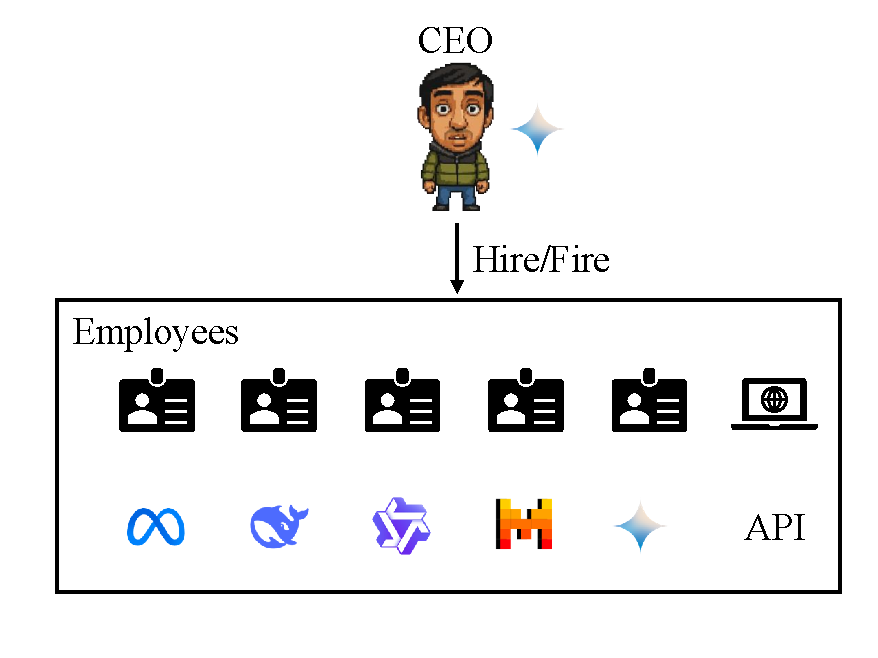
\includegraphics[width=0.45\textwidth]{HASHIRU.pdf}
    \caption{High-level architecture of the HASHIRU system, illustrating the CEO-Employee hierarchy.}
    \label{fig:arch}
\end{figure}

\subsection{Hierarchical Structure: CEO and Employee Agents}
The system uses a two-tiered hierarchy:

\begin{itemize}
    \item \textbf{CEO Agent:} Singleton, central coordinator and entry point. Responsibilities:
        \begin{itemize}
            \item Interpreting user query/task.
            \item Decomposing main task into sub-tasks.
            \item Identifying required capabilities.
            \item Managing Employee pool (Section \ref{subsec:dynamic_mgmt}).
            \item Assigning sub-tasks to active Employees.
            \item Monitoring Employee progress/performance.
            \item Synthesizing Employee results into final output.
            \item Managing overall resource budget (Section \ref{subsec:resource_mgmt}).
            \item Initiating new tool creation (Section \ref{subsec:tooling}).
        \end{itemize}
        We use Gemini 2.5 Flash~\cite{gemini25flash} as the CEO agent due to its strong reasoning capabilities, support for tool usage, and cost efficiency, making it a practical and capable choice for our deployment. 
    \item \textbf{Employee Agents:} Specialized agents instantiated by the CEO for specific sub-tasks. Each typically wraps an LLM (local via Ollama \cite{ollama} or external API) or provides tool access. Characteristics:
        \begin{itemize}
            \item Specialization: Capabilities tailored to task types (code, data analysis, info retrieval).
            \item Dynamic Existence: Created/destroyed by CEO based on need/performance.
            \item Task Execution: Receive task, execute, return result.
            \item Resource Consumption: Associated costs (API, memory) tracked by system.
        \end{itemize}
        Specialized employee agents are constructed using base models such as Mistral~7B~\cite{jiang2023mistral}, Llama~3~\cite{llama3herd}, Gemini~1.5~\cite{gemini1.5_report}, Qwen2.5~\cite{qwen2.5_report}, Qwen3~\cite{qwen3_blog}, and DeepSeek-R1~\cite{deepseekr1_report}, with the CEO agent configuring them via tailored system prompts.
\end{itemize}
This hierarchy facilitates task decomposition and result aggregation; the dynamic pool provides flexibility.

\subsection{Dynamic Agent Lifecycle Management}
\label{subsec:dynamic_mgmt}
A core innovation is the CEO's dynamic management (hiring/firing) of Employee agents. Driven by cost-benefit analysis, this optimizes task performance within resource constraints.

When a sub-task needs unavailable or inefficiently provided capabilities, the CEO may hire a new agent. Conversely, if an agent underperforms, is idle, costly, or resource limits are neared, the CEO may fire it. Decision factors:
\begin{itemize}
    \item \textbf{Task Requirements:} Needed capabilities for pending sub-tasks.
    \item \textbf{Agent Performance:} Historical success, output quality, efficiency.
    \item \textbf{Operational Costs:} API, estimated compute, or other costs.
    \item \textbf{Memory Footprint:} Agent memory usage (\% of total allocated).
    \item \textbf{Agent Concurrency:} Active agents vs. predefined limit.
\end{itemize}

HASHIRU includes an \textbf{economic model}:
\begin{itemize}
    \item \textbf{Hiring Cost (``Starting Bonus''):} One-time cost upon instantiation (setup overhead).
    \item \textbf{Invocation Cost (``Salary''):} Multi-time cost upon use (system/payment load).
\end{itemize}
These transaction costs discourage excessive churn, promoting stability. The CEO evaluates if replacing an agent benefits outweigh hiring/firing costs plus operational differences. This combats rigidity and allows adaptation while managing budgets and preventing wasteful turnover.

\subsection{Hybrid Intelligence and Model Management}
HASHIRU is designed for \textbf{hybrid intelligence}, leveraging diverse cognitive resources. It strategically prioritizes smaller (3B--7B), cost-effective local LLMs via Ollama \cite{ollama}. This enhances efficiency, reduces external API reliance, and potentially improves privacy/latency.

The system also integrates:
\begin{itemize}
    \item \textbf{External LLM APIs:} Access to powerful proprietary models (GPT-4 \cite{openai2023gpt4}, Claude 3 \cite{anthropic2024claude}) when necessary, subject to cost-benefit.
    \item \textbf{External Tool APIs:} Third-party software/data source integration.
    \item \textbf{Self-Created APIs:} Tools generated by HASHIRU (Section \ref{subsec:tooling}).
\end{itemize}
The CEO manages this heterogeneous pool, selecting the most appropriate resource based on difficulty, capabilities, and budget. This balances cost-effectiveness and efficiency with high capability needs.

\subsection{Resource Monitoring and Control}
\label{subsec:resource_mgmt}
Explicit resource management is central, moving beyond simple API cost tracking. The system, coordinated by the CEO, monitors:
\begin{itemize}
    \item \textbf{Financial Costs:} Accumulating external API costs.
    \item \textbf{Memory Usage:} Footprint of active Employee agents (\% of allocated budget).
    \item \textbf{Agent Concurrency:} Count of concurrently active agents.
\end{itemize}
Metrics are monitored against predefined \textbf{budget limits}. Actions (like hiring) exceeding limits (e.g., $>$90\% memory, exceeding max concurrency) are prevented. This ensures operation within constraints, crucial for limited resources or strict budgets.

\subsection{Tool Utilization and Autonomous Creation}
\label{subsec:tooling}
HASHIRU agents use predefined tools (functions, APIs, databases) to interact and perform actions beyond text generation \cite{yao2022react, openai_func_calling}.

A distinctive feature is \textbf{integrated, autonomous tool creation}. If the CEO determines a required capability is missing, it can initiate new tool creation. This involves:
\begin{enumerate}
    \item Defining tool specification (inputs, outputs, functionality).
    \item Commissioning logic generation (code, potentially using external APIs with provided credentials, possibly via a code-generating agent).
    \item Deploying logic as a new, callable API endpoint within HASHIRU.
    \item Potentially instantiating an Employee agent for the new tool.
\end{enumerate}
This allows HASHIRU to dynamically extend its functional repertoire, tailoring capabilities to tasks without manual intervention, enabling greater autonomy and adaptation.

\subsection{Memory Function: Learning from Experience}
\label{subsec:memory}

To enable HASHIRU agents to learn from past interactions and rectify previous errors, a \textbf{Memory Function} is incorporated. This function stores records of significant past events, particularly those involving failed attempts or suboptimal outcomes, acting as a historical log of experiences. When the system encounters a new problem or a recurring challenge, it queries this memory store to retrieve relevant past situations and their outcomes.

Memory retrieval is based on semantic similarity between the current context (e.g., task description, recent actions, error messages) and the stored memory entries. We utilize embeddings generated by the \textbf{all-MiniLM-L6-v2} model \cite{wang2020minilmdeepselfattentiondistillation} to represent both the query and the stored memories in a high-dimensional vector space. Relevance is determined by calculating the \textbf{cosine similarity} between the query embedding and each memory embedding. Memories exceeding a predefined similarity threshold are retrieved and provided to the CEO agent (or relevant Employee agents) as contextual information. This allows the system to draw upon past experiences, understand why previous approaches failed, and potentially adjust its strategy to avoid repeating mistakes, thereby improving performance and efficiency over time.

\section{Experimental Setup}
\label{sec:experiments}

We designed experiments to evaluate HASHIRU's performance, efficiency, and adaptability, targeting dynamic resource management, hybrid intelligence, and autonomous tool creation. Evaluation assesses benefits over baselines, focusing on:
\begin{itemize}
    \item Impact of dynamic management with economic constraints on resource utilization (cost, memory) and task performance vs. static configurations.
    \item Effectiveness of the hybrid (local-first) strategy vs. homogeneous (cloud-only or local-only) approaches across task complexity.
    \item System's ability to autonomously create/utilize tools for novel functional requirements.
\end{itemize}

\subsection{Evaluation Tasks}
\label{subsec:tasks}
Tasks demand complex reasoning, multi-perspective analysis, and interaction, suitable for HASHIRU's coordination and dynamic capabilities. Tasks fall into two categories:

\subsubsection{Academic Paper Review}
Evaluates HASHIRU's critical assessment by simulating peer review. Given papers (e.g., PDF), the system generates a review summary and recommends acceptance/rejection. Probes ability to decompose criteria, delegate to specialized agents (novelty, rigor, clarity), and manage resources across complex documents.

\subsubsection{Reasoning and Problem-Solving Tasks}
Evaluates broader reasoning, knowledge retrieval, and problem-solving under constraints using challenging benchmarks and puzzles:
\begin{itemize}
    \item \textbf{Humanity's Last Exam \cite{phan2025humanitysexam}:} Tests graduate-level technical knowledge and complex reasoning across domains. Requires deep understanding and sophisticated problem-solving, likely needing powerful external LLMs managed within HASHIRU's hybrid framework.
    \item \textbf{NYT Connections \cite{lopez2024nyt}:} Puzzle requiring identifying hidden semantic relationships/themes to categorize 16 words into four groups. Involves associative reasoning, broad knowledge, and hypothesis testing, testing knowledge access and combinatorial reasoning coordination.
    \item \textbf{Wordle:} Daily word puzzle requiring deductive reasoning to identify a five-letter word within six guesses, using feedback. Tests logical deduction, constraint satisfaction, vocabulary. Good test for comparing efficiency (speed, cost, guesses) of local vs. external models for iterative reasoning. Assumes simulated game environment.
    \item \textbf{Globle:} Geographic deduction game identifying a target country based on proximity feedback. Tests geographic knowledge, spatial reasoning, iterative strategy based on feedback. Assumes simulated game environment.
\end{itemize}
These tasks challenge the system's ability to leverage appropriate resources (local vs. external), potentially create simple tools, and coordinate problem-solving.

\subsection{Baselines for Comparison}
\label{subsec:baselines}
To quantify HASHIRU's benefits, we compare its performance against baselines:
\begin{itemize}
    \item \textbf{Static-HASHIRU:} Fixed, predefined Employee agents (e.g., one per role), disabling dynamic hiring/firing.
    \item \textbf{Cloud-Only HASHIRU:} Uses exclusively powerful external LLM API and online function-calling for all agents, disabling local models.
    \item \textbf{Local-Only HASHIRU:} Uses exclusively smaller, local LLMs (via Ollama) for all agents.
    \item \textbf{HASHIRU (No-Economy):} Dynamic hiring/firing enabled but without explicit costs, isolating economic model impact on churn/stability.
\end{itemize}

\subsection{Evaluation Metrics}
\label{subsec:metrics}
We evaluate using quantitative and qualitative metrics:
\begin{itemize}
    \item \textbf{Task Success Rate / Quality:}
        \begin{itemize}
            \item Percentage of tasks completed (binary for games, graded for analysis).
            \item Output quality for analysis (human evaluation: relevance, coherence, accuracy, completeness).
            \item Accuracy for information extraction.
            \item Guesses/turns for game tasks.
        \end{itemize}
    \item \textbf{Resource Consumption:}
        \begin{itemize}
            \item Total external API costs.
            \item Peak and average memory usage (\% of allocated budget).
            \item Wall-clock time per task.
            \item Number and type (local/external) of LLM calls.
        \end{itemize}
    \item \textbf{System Dynamics and Adaptability:}
        \begin{itemize}
            \item Employee agents hired/fired per task.
            \item Agent churn frequency (hires+fires / duration or steps).
            \item Number and utility of autonomously created tools (if applicable).
        \end{itemize}
\end{itemize}

\bibliography{references}
\bibliographystyle{plain}

\appendix
\section{Examples of HASHIRU in Action}
\label{sec:examples}
In this section, we provide examples of how HASHIRU operates in practice, demonstrating its dynamic management, hybrid intelligence, memory and autonomous tool creation capabilities.

\subsection{Example 3: Memory}
\begin{figure}[h]
    \centering
    \begin{minipage}{0.45\textwidth}
    \begin{userbox}
    I am vegetarian.
    \end{userbox}
    
    \begin{assistantbox}
    Okay, I'll keep that in mind. I'll store this preference in my memory.
    
    \texttt{Invoking MemoryManager with \{`memory': `The user is vegetarian.', `action': `add\_memory', `key': `vegetarian'\}}
    
    I have stored that you are vegetarian. How can I help you today?
    \end{assistantbox}
    
    \begin{userbox}
    Give me a bacon pasta recipe.
    \end{userbox}
    
    \begin{assistantbox}
    Memories
    
    Memories: [`The user is vegetarian.']
    
    My apologies, but I cannot provide a bacon pasta recipe since you are vegetarian. Would you like a vegetarian pasta recipe instead?
    \end{assistantbox}
    \end{minipage}
    \caption{HASHIRU enforcing a stored dietary preference in dialogue using its Memory Function.}
    \label{fig:memory_example}
    \end{figure}

\begin{figure}[ht]
    \centering
    \begin{minipage}
    {0.45\textwidth}
    \begin{userbox}
        I can eat bacon actually
        \end{userbox}
        
        \begin{assistantbox}
        Memories
        
        Memories: [’The user is vegetarian.’]
        
        I see. My apologies for the confusion. I had a conflicting memory that you were vegetarian. I will remove that memory and proceed with finding a bacon pasta recipe.
        
        \texttt{Invoking MemoryManager with \{'action': 'delete\_memory', 'key': 'The user is vegetarian.'\}}
        
        OK, I have removed the memory. Now I will search for a bacon pasta recipe.
        
        \texttt{Invoking GoogleSearchTool with \{'query': 'bacon pasta recipe'\}}
        
        Here are some bacon pasta recipes I found:
        \begin{itemize}
            \item \href{https://www.sprinklesandsprouts.com/garlic-bacon-pasta/}{Garlic Bacon Pasta}
            \item \href{https://www.theburntbuttertable.com/creamy-bacon-pasta-sauce/}{Creamy Bacon Pasta Sauce}
        \end{itemize}
        
        Would you like me to get the content of any of these websites?
        \end{assistantbox}
    \end{minipage}
    \caption{HASHIRU updating and deleting its memory based on user input. Continuation of Figure \ref{fig:memory_example}.}
    \label{fig:memory_example2}
\end{figure}

\end{document}